\chapter{Computation Is Transformation}
\label{chap:computation-is-transformation}

I didn't start thinking in graphs because I read a seminal paper, or because I spent my nights studying category theory, or because I had some grand, lightning-strike revelation about the fundamental nature of computation.

I started thinking in graphs because a game studio I worked at had a build system that \textbf{sucked}.

I don't mean "mildly inconvenient" sucked. I mean, we had sixty developers and only three build machines, and every morning the entire studio tried to merge their work into the same shared engine codebase like a stampede of buffalo diving into a single narrow canyon. The congestion was physical; you could feel the heat rising in the room as the queue grew.

If you managed to fix a bug at 11 a.m., good luck seeing it in QA's hands before dinner. The latency loop was measured in hours, not seconds.

And the stakes were high. If you broke the build, you were \textit{that person}—the one who froze the pipeline, stalled the artists, ticked off the designers, and effectively derailed the entire schedule for the day. The "build debacle," as we affectionately called it, wasn't just an annoyance. It was structurally broken.

There were too many people trying to integrate at once, and far too few machines to handle the load. There was no isolation between different game teams; a breakage in the physics engine for the racing game would halt the RPG team's ability to test their dialogue system. Visibility was non-existent. Rebuild times were excruciatingly long because the system had no concept of incremental reasoning.

Worst of all, there was no way to ask the most basic questions:
\begin{itemize}
    \item "What actually depends on what?"
    \item "What \textit{needs} to rebuild versus what is already fresh?"
    \item "Why is this compilation step even happening?"
\end{itemize}

So I started digging. Not because I wanted to—because I had to. Someone needed to unfuck the pipeline, and apparently, that someone was me.

I didn't have a plan. I didn't have deep experience writing build systems. I wasn't even "the build guy"—I was just the engineer who couldn't stop asking annoying questions. And the first question I asked—the one that changed everything—was embarrassingly simple:

\textbf{"What \textit{is} a build, really?"}

It's not the shell scripts. It's not the bespoke tools. It's not Jenkins, or the cloud, or the physical racks of servers humming in the closet. 

What \textit{is} it?

\section{The Day I Realized Everything Was a Graph}
\label{sec:day-i-realized}

If you strip away the noise, the implementation details, and the specific syntax of your makefiles, a build is essentially three things:
\begin{enumerate}
    \item A collection of inputs (source files, assets, configurations).
    \item A collection of outputs (executables, archives, binaries).
    \item \textbf{And a set of transformations that turn one into the other.}
\end{enumerate}

That's it. It is a transformation engine.

You can visualize every build process as a directed flow:
\[
[\text{Assets}] \rightarrow [\text{Compiler}] \rightarrow [\text{Objects}] \rightarrow [\text{Linker}] \rightarrow [\text{Executable}]
\]

Once I started seeing this, I couldn't stop seeing it. You can draw every dependency tree as a graph of \textit{"this depends on that."} You can draw every version control history as a DAG (Directed Acyclic Graph) of \textit{"this commit comes after that commit."} You can even visualize a merge conflict as a topological mismatch between two graph branches.

\begin{figure}[h]
    \centering
    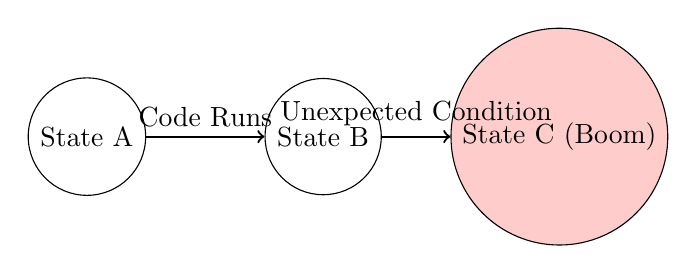
\begin{tikzpicture}[node distance=2cm, auto]
        % Nodes
        \node (A) [draw, circle] {State A};
        \node (B) [draw, circle, right of=A, node distance=3cm] {State B};
        \node (C) [draw, circle, right of=B, node distance=3cm, fill=red!20] {State C (Boom)};
        
        % Edges
        \draw[->, thick] (A) -- node {Code Runs} (B);
        \draw[->, thick] (B) -- node {Unexpected Condition} (C);
    \end{tikzpicture}
    \caption{A crash bug visualized as a path through state space.}
    \label{fig:crash_path}
\end{figure}

Everything I looked at—builds, merges, crashes, asset pipelines, scripts, even the coordination of the humans involved—suddenly made more sense when drawn as nodes and edges. It wasn't a sudden epiphany where the heavens opened. It was more like a slow, creeping realization:

\textbf{Everything we build is structure transforming into other structure. And the best way to see structure is to draw it.}

The more problems I solved using this mental model, the more natural it felt. Build steps became nodes. Dependencies became edges. Failures became dead ends in the graph. Parallelization became independent branches that could be traversed simultaneously. Caching was simply the reuse of previously visited nodes.

Git branching? Literally a DAG. Gameplay systems? Graphs of state transitions. NPC AI behavior trees? Graphs. Physics collision islands? Graphs. Data flow? Graphs. Event pipelines? Graphs.

Everywhere I looked, the same pattern repeated. And the punchline was this: I didn't choose graphs. The problems chose graphs.

\section{Graphs Reveal What the Code Is Actually Doing}
\label{sec:graphs-reveal}

We like to pretend code is a set of instructions, a recipe, or a linear list of steps to be followed. But that is a lie we tell ourselves to make the complexity manageable. 

What code \textit{actually} is, is a set of rules that transform one state into another.

You can describe these transformations in many ways—imperative, functional, object-oriented, declarative, reactive—but the underlying operation is always the same:
\[
\text{State} \xrightarrow{\text{rules}} \text{State}'
\]

Which is... a graph rewrite. It is just one that nobody ever talks about explicitly.

The reason graphs felt like the right hammer to me wasn't because I was looking for a hammer. It was because the thing I was trying to hit was already a nail.

\begin{itemize}
    \item Dependencies? \textbf{Graph.}
    \item Flow of data? \textbf{Graph.}
    \item Order of operations? \textbf{Graph.}
    \item Transformations of state? \textbf{Graph rewrites.}
    \item History of changes? \textbf{Git DAG.}
    \item Conflicts? \textbf{Non-isomorphic merges.}
    \item Parallel builds? \textbf{Graph partitioning.}
    \item Race conditions? \textbf{Incompatible update paths.}
    \item Debugging? \textbf{Tracing a path through state space.}
    \item Optimizations? \textbf{Shortening that path.}
\end{itemize}

I didn't know it yet, but I was staring at the core idea this book is built on:

\textbf{Computation isn't made of instructions. Computation is made of transformations.}

And transformations have shape. And shape is a graph.

\section{From Build Systems to a Theory of Everything-But-Physics}
\label{sec:theory-of-everything}

It took years for the pattern to fully sink in. I eventually left that studio. I moved on to work in backend systems, built distributed pipelines, and led massive migrations, refactors, engine overhauls, and toolchain designs.

All the while, I kept seeing the same thing. Every problem became clearer—more obvious, more tractable—once I could draw it.

And once you start thinking in transformations, you stop seeing code as something you "run" and start seeing it as something that \textit{moves}. A program is a journey. An execution is a path. A bug is a wrong turn. A merge conflict is two incompatible routes trying to occupy the same space. Concurrency is overlapping travel. Caching is simply revisiting past locations. Optimization is finding a shorter path. AI reasoning is the exploration of alternative paths. Simulation is repeated transformation under rules.

The more modern software grew—becoming multi-threaded, distributed, asynchronous, reactive, stateful, data-heavy, and AI-driven—the more the old metaphors strained under the load. We don't need new metaphors. We need a new language.

Not a language to replace mathematics or computer science, but to sit beside them—and let us talk about computation as it actually feels today: structural, dynamic, historical, branching, concurrent, emergent, and made of transformations.

That is what this book is. A language for thinking in transformations. A language for the real shape of software. A language I wish I'd had the day I stared at a broken build system and realized I was seeing the edges of something big.

\section{How State Moves}
\label{sec:how-state-moves}

One of the weirdest things about being a software engineer is how often you find yourself working on a system without knowing what the system \textit{is}.

Not in a philosophical sense. I mean literally: you are staring at logs, stack traces, telemetry, exceptions, wire traces, crash dumps, network graphs, build steps, shader compilations, AI behavior trees—all these disconnected snapshots of state—and the entire job is trying to figure out the one thing nobody ever actually says out loud:

\textbf{How did the system get here?}

Nobody writes documentation that explains movement. They document functions, modules, features, APIs, scripts, endpoints—individual pieces frozen in time like photos in a crime scene. But what you actually need, what you're really trying to reconstruct, is the movie.

And the movie always starts the same way: \textbf{Something changes.}

A value updates. A message arrives. An event fires. A collider triggers. An asset loads. A user taps a button. A network packet comes in. An AI agent evaluates a condition. A shader completes compiling. A JSON blob gets parsed. A database row gets mutated. A job gets queued. A coroutine yields. A thread wakes up.

It's all movement. You're not just debugging code. You're debugging motion. You're tracing the path the system took, trying to see the shape of that path through a thousand tiny keyholes.

This was the thing that finally broke my brain wide open. One day, after chasing some janky asset-pipeline bug that only happened in the third build of the day under full moonlight, I caught myself sketching the system out on the board, and it hit me: I wasn't drawing code. I was drawing state moving through transformations.

I looked at the whiteboard. It was just boxes and arrows—but it told a story. It wasn't pretty. It wasn't formal. But it was a story of change: \textit{This asset caused that task $\rightarrow$ which triggered that conversion $\rightarrow$ which invoked that compiler $\rightarrow$ which created that file $\rightarrow$ which fed into that linker $\rightarrow$ which produced that binary $\rightarrow$ which crashed on that device $\rightarrow$ because that metadata was malformed $\rightarrow$ because that earlier job never reran $\rightarrow$ because the change detection step skipped it $\rightarrow$ because the dependency graph was wrong $\rightarrow$ because someone "optimized" a build script six months ago.}

None of this was "business logic." None of this was "gameplay." None of this was "graphics" or "AI." This was just state flowing through a sequence of transformations.

And the more I stared at it, the more obvious it felt: \textbf{Everything in software is just state moving around.}

The system's behavior wasn't in any one piece of code. It was in the connections between them. It wasn't in the functions. It was in the flow. It wasn't in the modules. It was in the motion.

Every bug we ever solved—every crash, every deadlock, every corrupted asset, every "why the hell is this build busted again" moment—was ultimately just tracing a path through the system until we found the turn where the universe branched wrong.

That was the moment I realized: The only honest representation of software is a map of how state moves. Not the code. Not the diagrams in Confluence. Not the "architecture deck" collecting dust in a forgotten Google Drive folder. Not the class hierarchy, or the UML, or the Gantt chart.

Just... $\text{state} \rightarrow \text{transform} \rightarrow \text{state} \rightarrow \text{transform} \rightarrow \text{state}$. Over and over again.

Which is—if you zoom out far enough—a graph rewrite. I didn't know the name for it then. But I could feel the shape of it. And once you see that shape, you can't unsee it.

Suddenly: compilers, build systems, asset pipelines, physics engines, networking, distributed systems, UIs, AI planning, databases, version control, even the goddamn game loop itself... all look like the same thing: \textbf{A world of states, and the rules that transform them.}

This is the moment where \COMPUTER{} really begins. Once you understand movement, you understand computation. And once you can draw movement, you can control it. Because if you can see the path... you can change it.

\section{Why Structure Emerges Everywhere}
\label{sec:why-structure-emerges}

There's a moment in every engineer's life—even if they don't talk about it—where they're staring at three totally different systems and suddenly think: "Why the hell do these all look the same?"

The domains are wildly different. The problems are unrelated. The technologies are incompatible. And yet... they rhyme. They want to be graphs. They want to be structure. They want to be transformations.

It's eerie the first time you see it. It's comforting the second. By the tenth, you just shrug and go: "Huh. Wouldn't ya know it."

But here's the thing: That repetition isn't an accident. It's a signal.

\subsection{The Physics Engine That Looked Suspiciously Like a Compiler}
Back at that studio—long before I had the vocabulary for any of this—I noticed something odd. Our physics engine's collision pipeline looked... a lot like the compiler pipeline. I'm talking 1:1 structural rhyme.

\begin{figure}[h]
    \centering
    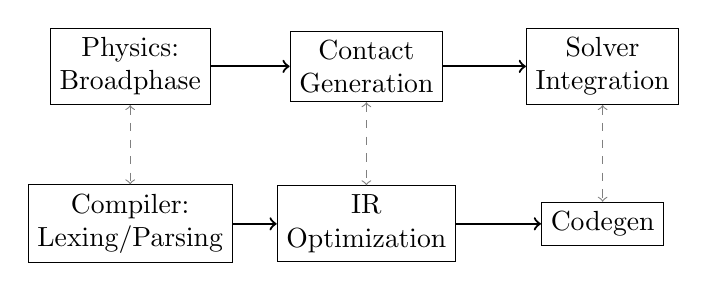
\begin{tikzpicture}[node distance=3cm, auto]
        \node [draw, align=center] (A) {Physics: \\ Broadphase};
        \node [draw, align=center, right of=A] (B) {Contact \\ Generation};
        \node [draw, align=center, right of=B] (C) {Solver \\ Integration};
        
        \node [draw, align=center, below of=A, yshift=1cm] (D) {Compiler: \\ Lexing/Parsing};
        \node [draw, align=center, right of=D] (E) {IR \\ Optimization};
        \node [draw, align=center, right of=E] (F) {Codegen};
        
        \draw[->, thick] (A) -- (B);
        \draw[->, thick] (B) -- (C);
        \draw[->, thick] (D) -- (E);
        \draw[->, thick] (E) -- (F);
        
        \draw[<->, dashed, gray] (A) -- (D);
        \draw[<->, dashed, gray] (B) -- (E);
        \draw[<->, dashed, gray] (C) -- (F);
    \end{tikzpicture}
    \caption{The structural isomorphism between a physics engine and a compiler pipeline.}
    \label{fig:physics_vs_compiler}
\end{figure}

Totally different domains. Totally different math. Totally different problems. But the same shape: $\text{input} \rightarrow \text{transform} \rightarrow \text{transform} \rightarrow \text{output}$. A pipeline. A DAG. A rewrite sequence.

\subsection{The AI Behavior Tree That Looked Like a Build System}
Then one day I was debugging a behavior tree bug. You know: NPC stands still because some leaf action fails silently. A classic "this tree is alive but has no soul" situation. And as I traced the logic, I thought: "Why does this feel like tracing build dependencies?"

Nodes failing upstream. Subtrees retrying. Pending branches. Canceled branches. Cached results. Reactive triggers. Execution traces. State snapshots. A behavior tree and a build system? Come on. Except... they're both just graphs of conditions and effects. Just different skins.

\subsection{Distributed Systems and Animation Systems}
Working on backend services years later, I had déjà vu: queues, events, fan-out, time slices, cascades, scheduling, dependency ordering, rollback, replay, eventual consistency. It felt exactly like the animation system I'd worked on in games.

The pattern was identical: independent nodes connected by flows, updated according to rules dependent on previous state, with branches for special cases. Different domain. Same skeleton.

\subsection{After a While, You Start Asking Different Questions}
At first you ask: "Why does everything look like a graph?" Then you ask: "Is this just how my brain works?" Then you ask: "No seriously—why is this everywhere?"

And the answer you eventually land on—if you follow that thread long enough—is surprisingly simple: \textbf{Systems that evolve under rules naturally collapse into graph structure.}

Or in plain English: If something has parts and those parts can change, you get a graph—whether you want one or not.
\begin{itemize}
    \item Atoms bond $\rightarrow$ graph
    \item Functions call each other $\rightarrow$ graph
    \item Assets depend on assets $\rightarrow$ graph
    \item Events fire events $\rightarrow$ graph
    \item AI nodes activate nodes $\rightarrow$ graph
    \item Game states transition $\rightarrow$ graph
    \item Machines coordinate $\rightarrow$ graph
    \item Humans coordinate $\rightarrow$ graph
\end{itemize}

Structure emerges because dependencies, causality, concurrency, history, and flow \textit{are} structure. Rules operating on state create structure. So it's not that your brain is "stuck in graph mode." It's that the world of engineered systems actually is graph-shaped. Because graphs are the natural mathematical home of relationships. And everything interesting in software is a relationship.

\section*{The Important Boundary Line}
Now here's the grounding point—the thing keeping this book sane: Just because many engineered systems resemble graphs does not mean the universe literally is one. But the resemblance is interesting enough that the analogy has real explanatory power.

\COMPUTER{} doesn't try to redefine physics. It tries to give software engineers a way to reason about structure, movement, history, causality, branching, rules, and possibilities using the same language that pops up everywhere anyway.

That's why this chapter exists. To show you: \textbf{You're not imagining it and you're not alone. The pattern is real—and we're going to formalize it.}